\section{Primer on data structures \& metadata formats}

\begin{frame}{TEI, now what?}
\metroset{block=fill}
    Why are we doing this workshop? The motivation from our abstract:
    \begin{itemize}
        \item \punkti the Text Encoding Initiative (TEI) for XML has become the gold standard for scholarly editions of texts.
        \item But what happens after an edition is encoded in TEI? 
    \end{itemize}
    
    \begin{block}{Goals for the next session}
    \begin{enumerate}
        \item There are many different types of data. They get stored in different structures. 
        \item Why XML and not something else?
        \item What else is there? 
        \item \textbf{Also:} some metadata literacy!
    \end{enumerate}
    \end{block}
\end{frame}

%------------------------------------------------------------------------------
\begin{frame}{Digital data representation}
\metroset{block=fill}\small
$\to$ i.e. \alert{machine processable}

\begin{columns}
\column{0.62\textwidth}
\begin{block}{Digital representations}
    \begin{itemize}\footnotesize
        \item \textbf{Images} 
        \begin{itemize}
            \item raster graphics (\texttt{.png}, \texttt{.jpeg}) 
            \item vector graphics (\texttt{.svg})
        \end{itemize}
        \item \textbf{Text}
        \begin{itemize}
            \item plain text (\texttt{.txt})
            \item formatted text (\texttt{.docx}, \texttt{.rtf}, \texttt{.xml}, \texttt{.tex})
        \end{itemize}
        \item \textbf{Lists \& tables} (\texttt{.csv}, \texttt{.xlsx})
        \item \textbf{Sound} (\texttt{.wav}, \texttt{.midi})
        \item \textbf{Objects:} (Simulated) 3D view, abstracted representation by description and images
    \end{itemize}
\end{block}

\column{0.35\textwidth}
\begin{block}{Further types}
\begin{itemize}\footnotesize
    \item \textbf{markup languages} (\texttt{.xml}, \texttt{.html}, etc.)
    \item \textbf{data objects} (\texttt{.json}, etc.) 
    \item \textbf{graphs / graph databases} (\texttt{.rdf}, etc.)
    \item \textbf{relational databases} $\to$ SQL 
\end{itemize}
\end{block}
\end{columns}

\end{frame}


%------------------------------------------------------------------------------
\begin{frame}[fragile]{Data structures: Graphs}
\metroset{block=fill}
  \begin{columns}[T,onlytextwidth]
    \column{0.37\textwidth}
    Applications
      \begin{itemize}\footnotesize
          \item \textbf{Resource Description Framework (RDF):} 
          \begin{itemize}\footnotesize
              \item e.g. Blazegraph (Graph-DB)
              \item Query: SPARQL
          \end{itemize}
          \item Labeled Property Graphs
          \begin{itemize}\footnotesize
              \item e.g. Neo4j (Graph-DB)
              \item Query: Cypher
          \end{itemize}
      \end{itemize}
      
      \begin{block}{}
        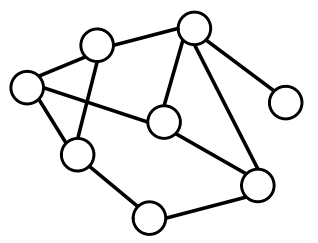
\includegraphics[width=0.97\textwidth]{img/graph.png}
      \end{block}


    \column{0.6\textwidth}
    RDF/Turtle-Notation (\texttt{.ttl})
\begin{turtlecode}
@prefix ex: <http://example.com/#> .

ex:Graz a ex:city;  
ex:name "Graz" ; 
ex:inhabitants 288806 ; 
ex:location [ ex:lat 47.4; ex:long 5.26 ] .

ex:Wien a ex:city;  
ex:name "Wien" ; 
ex:inhabitants 1897491 ; 
ex:location [ ex:lat 47.12; ex:long 16.22 ] .
\end{turtlecode}

SPARQL query
\begin{sparqlcode}
@prefix ex: <http://example.com/#> .

SELECT ?name, ?population
WHERE {
    ?city ex:inhabitants ?population .
}
\end{sparqlcode}

  \end{columns}
\end{frame}

%------------------------------------------------------------------------------
\begin{frame}[fragile]{Data structures: tabular data / relational databases}
%\metroset{block=fill}
  \begin{columns}[T,onlytextwidth]
    \column{0.3\textwidth}
    Applications
      \begin{itemize}\footnotesize
          \item e.g. SQLite, MySQL (relational dbs) 
          \item Query: SQL 
      \end{itemize}
      \bigskip 
      
      \begin{block}{}
        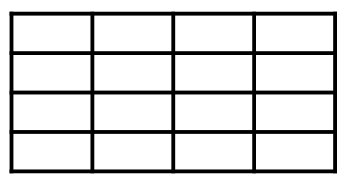
\includegraphics[width=0.97\textwidth]{img/tabelle.png}
      \end{block}


    \column{0.65\textwidth}
SQL query
\begin{sqlcode}
CREATE TABLE "places" (
 "name" TEXT,
 "population" INTEGER,
 "longitude" REAL,
 "latitude" REAL,
 PRIMARY KEY("name")
);

INSERT INTO places 
VALUES 
('Graz', 288806, 47.066667, 15.433333), 
('Wien', 1897491, 48.208174, 16.373819);
\end{sqlcode}
\footnotesize
(name, population, longitude, latitude) 

  \end{columns}
\end{frame}


%------------------------------------------------------------------------------
\begin{frame}[fragile]{Data structures: tree hierarchy 1 / JSON}
%\metroset{block=fill}
    Applications: \textbf{JavaScript Object Notation (JSON)}
          \begin{itemize}\footnotesize
              \item e.g. MongoDB
              \item no standardized query language, just JavaScript (\texttt{.js})
          \end{itemize}

\begin{block}{}      
\begin{flushright}
        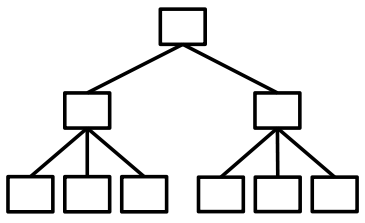
\includegraphics[width=0.25\textwidth]{img/baumstruktur.png}
\end{flushright}
\end{block}

JSON \& JS (\href{https://www.w3schools.com/js/js_json_intro.asp}{w3s})
\begin{jscode}
'{"name": "John", "age": 30, "car": null, 
  "tree" : [
    "key": "value"
  ]
}'
const obj = JSON.parse('{"name":"John", "age":30, "city":"New York"}');
obj.age = obj.age.toString();
\end{jscode}

\end{frame}


%------------------------------------------------------------------------------
\begin{frame}[fragile]{Data structures: tree hierarchy 2 / XML}
%\metroset{block=fill}
  \begin{columns}[T,onlytextwidth]
    \column{0.33\textwidth}
    Applications: \textbf{eXtensible Markup Language (XML):}
          \begin{itemize}\footnotesize
              \item DBs: eXist, BaseX 
              \item Query: 
              XPath (\href{https://www.w3schools.com/xml/xpath_intro.asp}{w3s}) and XQuery (\href{https://www.w3schools.com/xml/xquery_example.asp}{w3s})
          \end{itemize}
          \bigskip

      \begin{block}{}
        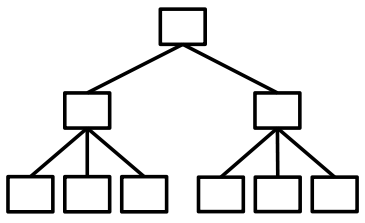
\includegraphics[width=0.95\textwidth]{img/baumstruktur.png}
      \end{block}

    \column{0.65\textwidth}
\begin{xmlcode}
<!-- books.xml -->
<?xml version="1.0" encoding="UTF-8"?>
<bookstore>
  <book>
    <title lang="en">Harry Potter</title>
    <author>J K. Rowling</author>
    <year>2005</year>
    <price>29.99</price>
  </book>
  <book>
    <title lang="en">Learning XML</title>
    <price>39.95</price>
  </book>
</bookstore>

<!-- XQuery -->
for $x in doc("books.xml")/bookstore/book
where $x/price>30
order by $x/title
return $x/title

<!-- XPath -->
//title[@lang='en']
/bookstore/book[price>35.00]
\end{xmlcode}

  \end{columns}
\end{frame}
%------------------------------------------------------------------------------

%------------------------------------------------------------------------------
\begin{frame}[fragile]{Data structures: tree hierarchy 3 / web pages (HTML)}
%Datentypen, die man vielleicht kennen sollte
%\metroset{block=fill}
  \begin{columns}[T,onlytextwidth]
    \column{0.47\textwidth}
    HTML (\href{https://www.w3schools.com/html/default.asp}{w3s}) -- structure
\begin{htmlcode}
<!DOCTYPE html>
<html>
 <head>
   <title>Page Title</title>
 </head>
 <body>
  <h1>This is a Heading</h1>
  <p>This is a paragraph.</p>
 </body>
</html>
\end{htmlcode}

      
      \begin{block}{}
        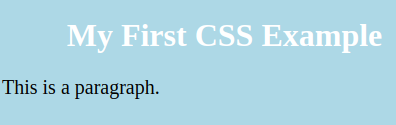
\includegraphics[width=0.97\textwidth]{img/css-example.png}
      \end{block}


    \column{0.47\textwidth}

CSS in HTML (\href{https://www.w3schools.com/css/default.asp}{w3s}) -- rendering
\begin{htmlcode}
<!DOCTYPE html>
<html>
  <head>
    <style>
body {
  background-color: lightblue;
}
h1 {
  color: white;
  text-align: center;
}
p {
  font-family: verdana;
  font-size: 20px;
}
    </style>
  </head>
  <body>
    <h1>My First CSS Example</h1>
    <p>This is a paragraph.</p>
  </body>
</html>
\end{htmlcode}

  \end{columns}
\end{frame}
%------------------------------------------------------------------------------

\begin{frame}{Why so many data formats?}
\metroset{block=fill}\small
Different data formats (\& standards) focus on different aspects \& have different goals:
\begin{enumerate}
\item \textbf{text-based}
	\begin{itemize}\scriptsize
	\item Text Encoding Initiative (\textbf{TEI})
	\item Extensible Hypertext Markup Language (\textbf{XHTML} = XML-compliant HTML)
	\item Open Document Format for Office Applications (\textbf{ODF})
	\end{itemize}
\item \textbf{page-based}
	\begin{itemize}\footnotesize
	\item \textbf{\TeX{} / \LaTeX{}}
	\item \textbf{XSL-FO} (XSL Formatting Objects, discontinued)
	\end{itemize}
\item \textbf{ontology-based}
	\begin{itemize}\scriptsize
	\item Resource Description Framework (\textbf{RDF}) \& RDF Schema (\textbf{RDFS})
	\item Web Ontologie Language (\textbf{OWL})
	\item Simple Knowledge Organisation System (\textbf{SKOS})
	\item Conceptual Reference Model (\textbf{CIDOC-CRM})
	\end{itemize}
\item \textbf{digital archiving / digital objects}
	\begin{itemize}\scriptsize
	\item Dublin Core Metadata Initiative (\textbf{DCMI}), known as Dublin Core (\textbf{DC})
	\item Metadata Encoding and Transmission Standard (\textbf{METS})
	\item Metadata Object Description Schema (\textbf{MODS})
	\item Encoded Archival Description (\textbf{EAD})
	\item Charters Encoding Initiative (\textbf{CEI})
	\end{itemize}
\end{enumerate}

% Konzepte für Protokolle und Constraints: SOAP (Simple Object Access Protocol), XACML (Extensible Access Control Markup Language)
\end{frame}
%---------------------------------

\begin{frame}{A primer on metadata}
\metroset{block=fill}\small
\begin{columns}
\column{0.38\textwidth}
\begin{block}{What are metadata?}
\begin{itemize}
\item „data about data“
\begin{enumerate}\footnotesize
\item data about containers of data = \textbf{structural metadata}
\item data about the content represented by data = \textbf{descriptive metadata}
\end{enumerate}
\item functions:
\begin{enumerate}\footnotesize
\item descriptive
\item administrative
\item technical
\item use
\end{enumerate}
\end{itemize}
\end{block}

\column{0.58\textwidth}
\begin{block}{}
There are standards for the description of metadata (and many are XML-based), e.g.
\begin{itemize}\scriptsize
\item Machine-Readable Cataloging (\textbf{MARC})
\item Metadata Object Description Schema (\textbf{MODS})
\item Encoded Archival Description (\textbf{EAD})
\item Lightweight Information Describing Objects (\textbf{LIDO})
\item Collective Description of Works of Art (\textbf{CDWA}) / Visual Research Association (\textbf{VRA})
\item Europeana Metadata Model (\textbf{EDM})
\item Resource Description Framework (\textbf{RDF})
\item Metadata Encoding \& Transmission Standard (\textbf{METS})
\item Dublin Core (\textbf{DC})
\item Functional Requirements for Bibliographic Records (\textbf{FRBR})
\item the \texttt{<teiHeader>} has metadata\dots
\end{itemize}
\end{block}


\end{columns}
{\scriptsize \href{http://dixit.uni-koeln.de/wp-content/uploads/2015/04/Camp2-18-Georg_Vogeler_-_Metadata__talk.pdf}{Slides on metadata in DH with more information}}
\end{frame}

%---------------------------------
\begin{frame}[fragile,allowframebreaks]{Dublin Core (DC)}
\metroset{block=fill}

\begin{columns}
\column{0.48\textwidth}
\begin{block}{What is the DC?}
\begin{itemize}\footnotesize
    \item founded in Dublin (Ohio) in 1995
    \item \textbf{two levels:} simple (15 elements) \& qualified (additional \texttt{Audience}, \texttt{Provenance} and \texttt{RightsHolder})
    \item \textbf{classes of terms:} elements (nouns) \& qualifiers (adjectives).
    \item \href{https://www.dublincore.org/specifications/dublin-core/dcmes-xml/}{can be expressed in RDF/XML}
    \item each element is optional \& can be repeated
    \item also: \href{https://www.dublincore.org/specifications/dublin-core/dcmi-terms/}{dc:terms}
\end{itemize}
\end{block}

\column{0.48\textwidth}
\begin{block}{}
\begin{quote}
    \textbf{The Dublin Core™ metadata standard} is a simple yet effective\textbf{ element set for describing a wide range of networked resources.} \punkti 
    Another way to look at Dublin Core™ is as a ``small language for making a particular class of statements about resources''. In this language, there are two classes of terms -- \textit{elements} (nouns) and \textit{qualifiers} (adjectives) -- which can be arranged into a simple pattern of statements. 
    
    (\href{https://www.dublincore.org/specifications/dublin-core/usageguide/#whatis}{source})
\end{quote}
\end{block}
\end{columns}

\framebreak

\begin{columns}
\column{0.23\textwidth}

\begin{block}{The Core}\footnotesize
i.e. \href{https://www.dublincore.org/specifications/dublin-core/usageguide/elements/}{the elements}:
\begin{enumerate}\scriptsize
    \item title
    \item subject
    \item description
    \item type 
    \item source 
    \item relation 
    \item coverage
    \item creator
    \item publisher
    \item contributor
    \item rights
    \item date 
    \item format
    \item identifier 
    \item language
\end{enumerate}
\end{block}

\column{0.75\textwidth}

\begin{block}{Qualified}
\begin{enumerate}\scriptsize
    \item (audience)
    \item (provenance)
    \item (rights holder)
\end{enumerate}
\end{block}
\begin{xmlcode}
<rdf:RDF 
  xmlns:rdf="http://www.w3.org/1999/02/22-rdf-syntax-ns#"
  xmlns:dc="http://purl.org/dc/elements/1.1/">

   <rdf:Description rdf:about="http://media.example.com
                               /audio/guide.ra">
      <dc:creator>Rose Bush</dc:creator>
      <dc:title>A Guide to Growing Roses</dc:title>
      <dc:description>Describes process for 
        planting and nurturing different kinds 
        of rose bushes.</dc:description> 
      <dc:date>2001-01-20</dc:date>
   </rdf:Description> 
</rdf:RDF>
\end{xmlcode}
{\scriptsize Note the two namespaces \texttt{rdf:} and \texttt{dc:}.}
\end{columns}
\end{frame}

%---------------------------------------------

\begin{frame}[fragile]{Metadata Encoding and Transmission Standard (METS)}
\metroset{block=fill}
\begin{columns}
\column{0.55\textwidth}
\begin{block}{METS}\footnotesize
\begin{itemize}
\item tool for encoding digital library objects
\item container format for documents in which contents of different formats can be integrated 
\item also describes relationships between objects
\item describes logical and physical structure of an object
\item also contains descriptive (bibliographical) and administrative metadata
\item relatively simple and straightforward
\item supports a wide range of materials 
\item \href{https://www.loc.gov/standards/mets/mets-present.html}{<website>} \& \href{https://www.loc.gov/standards/mets/presentations/METS.ppt}{more info here}
\item DFG-Viewer: \protect\url{http://dfg-viewer.de/}
\end{itemize}
\end{block}
\column{0.41\textwidth}\small 
Only structural map is required.
\begin{xmlcode}
<mets>
  <metsHdr/>
  <dmdSec/>
  <amdSec/>
  <fileSec/>
  <structMap/>
  <structLink/>
  <behaviorSec/>
</mets>
\end{xmlcode}

%\protect\url{http://www.loc.gov/standards/mets/}

\begin{block}{Goals}
\begin{itemize}\scriptsize
    \item link/summarize related metadata
    \item e.g. link related images to text
    \item organize data
    \item provide usage metadata
\end{itemize}
\end{block}

\end{columns}
\end{frame}


%---------------------------

\begin{frame}[fragile]{Metadata Object Description Schema (MODS)}
\metroset{block=fill}
\begin{columns}
\column{0.32\textwidth}
\begin{block}{MODS}\scriptsize
\begin{itemize}
\item can represent the major elements from a MARC record
\item[$\to$] represents key bibliographic data in easily understandable names
\item[$\to$] easier to understand than MARC (for the uninitiated)
\item bridges the gap between library application and bibliographic source that don't make use of cataloging metadata formats
\item richer than the Dublin Core (DC) but less detailed than MARC
\item partially backwards compatible with MARC
\end{itemize}
\end{block}
\column{0.66\textwidth}
\begin{xmlcode}
<mods:mods xmlns:mods="http://www.loc.gov/mods/v3">    
  <mods:titleInfo>
    <mods:nonSort>The </mods:nonSort>
    <mods:title>
      1946 Library of Congress recital
    </mods:title>
  </mods:titleInfo>
  <mods:relatedItem type="constituent" 
                    ID="DMD_disc01_tr001">
    <mods:titleInfo type="uniform">
      <mods:partName>Chaconne von Vitali
        </mods:partName>
    </mods:titleInfo>
  </mods:relatedItem>
  <mods:identifier type="lccn">99594334
    </mods:identifier>
</mods:mods>
\end{xmlcode}
Code example from \href{http://www.digitalhumanities.org/dhq/vol/3/3/000064/000064.html}{here}.
\end{columns}
\end{frame}


%---------------------------------

\begin{frame}[fragile]{Encoded Archival Description (EAD)}
\metroset{block=fill}\small
\begin{columns}
\column{0.2\textwidth}
\begin{block}{EAD}
is a standard for encoding descriptive information regarding archival records
\end{block}

\href{https://www.loc.gov/ead/tglib/appendix_c.html}{example EAD} \& \href{https://en.wikipedia.org/wiki/Encoded_Archival_Description}{Wikipedia} (source of the example)

\column{0.78\textwidth}
\begin{xmlcode}
<eadheader>
   <eadid countrycode="us" identifier="bachrach_lf">
     bachrach_lf</eadid>
   <filedesc>
      <titlestmt>
         <titleproper encodinganalog="Title">
          Louis Fabian Bachrach Papers</titleproper>
         <subtitle>An inventory of his papers at 
           Blank University</subtitle>
         <author encodinganalog="Creator">Mary Smith</author>
      </titlestmt>
      <publicationstmt>
         <publisher encodinganalog="Publisher">
           Blank University</publisher>
         <date encodinganalog="Date" normal="1981">
           1981</date>
      </publicationstmt>
   </filedesc>
   <profiledesc>
      <creation>John Jones
         <date normal="2006-09-13">13 Sep 2006</date>
      </creation>
   </profiledesc>
</eadheader>
\end{xmlcode}
\end{columns}
\end{frame}



%---------------------------------
\begin{frame}[fragile]{Charters Encoding Initiative (CEI)}
\metroset{block=fill}
\begin{columns}
\column{0.35\textwidth}
\begin{block}{CEI}\footnotesize
considers the possibilities of a standard to encode medieval and early
modern charters with XML. 
\begin{itemize}\scriptsize
    \item implements the \emph{Vocabulaire Internationale de Diplomatique} 
    \item founded in 2004
    \item \href{https://www.monasterium.net/mom/home}{MOM-CA}, the collaborative charter archive of \href{https://www.icar-us.eu/en/cooperation/online-portals/monasterium-net/}{Monasterium.net} works with CEI
    \item \href{https://www.cei.lmu.de/}{<website>} \& \href{https://www.cei.lmu.de/examples/PS_Warenkorb.xml}{an example}. Also: \href{http://telota.bbaw.de/constitutiones/data/texts/600202b.xml}{the example below}.
\end{itemize}
\end{block}
\column{0.62\textwidth}
\begin{xmlcode}
<text type="charter">
  <idno>600202b</idno>
  <chDesc id="a">
    <head>Prag, 1360 Febr. 2.</head>
      <issued>
         <placeName>Prag</placeName>
         <date>1360-02-02</date>
      </issued>
      <abstract>
         <p> Karl verspricht Ludwig ...
         </p>
      </abstract>
      <witList>
         <witness sigil="B">
            Brandenburgisches LHA Potsdam 
            “Rep. 37 Hohennauen Nr. 683, 
            fol. 225” (18. Jh.)
         </witness>
      </witList>
      <diplomaticAnalysis>
         <bibl type="D">Fidicin, 42...</bibl>
      </diplomaticAnalysis>
   </chDesc> <tenor> </tenor>
</text>
\end{xmlcode}
\end{columns}
\end{frame}



%-------------------------------------------------------------------
\begin{frame}[fragile]{Resource Description Framework (RDF)}
\metroset{block=fill}
\begin{columns}
\column{0.4\textwidth}
\begin{block}{RDF}
\begin{itemize}\small
\item framework for describing resources in the World Wide Web
\item can contain metadata
\item language of the `Semantic Web' (web 3.0) -- makes things machine-processable
\item \href{https://www.w3.org/TR/rdf-schema/}{RDF Schema (RDFS)} offers Classes and Properties
\end{itemize}
\end{block}
\column{0.58\textwidth}
RDF/ turtle notation (\texttt{.ttl}) example from before
\begin{turtlecode}
@prefix ex: <http://example.com/#> .

ex:Graz a ex:city;  
ex:name "Graz" ; 
ex:inhabitants 288806 ; 
ex:location [ ex:lat 47.4; ex:long 5.26 ] .
\end{turtlecode}
\end{columns}
\end{frame}

%---------------------------------
\begin{frame}[fragile]{Simple Knowledge Organization System (SKOS)}
\metroset{block=fill}
\begin{columns}
\column{0.3\textwidth}
\begin{block}{SKOS}\footnotesize
RDF vocabulary for representing semi-formal \emph{knowledge organization systems} (KOSs), such as thesauri, taxonomies, classification schemes and subject heading lists.

$\to$ less rigorous than the logical formalism of ontology languages such as OWL
\end{block}
(\href{https://www.w3.org/TR/skos-primer}{SKOS primer})
\column{0.68\textwidth}
\begin{turtlecode}
@prefix skos: 
  <http://www.w3.org/2004/02/skos/core#> .
@prefix rdf: 
  <http://www.w3.org/1999/02/22-rdf-syntax-ns#> .
@prefix rdfs: 
  <http://www.w3.org/2000/01/rdf-schema#> .
@prefix owl: <http://www.w3.org/2002/07/owl#> .
@prefix dct: <http://purl.org/dc/terms/> .
@prefix foaf: <http://xmlns.com/foaf/0.1/> .
@prefix ex: <http://www.example.com/> .
@prefix ex1: <http://www.example.com/1/> .
@prefix ex2: <http://www.example.com/2/> .

ex:animals rdf:type skos:Concept;
  skos:prefLabel "animals"@en;
  skos:narrower ex:mammals.
  
ex:mammals rdf:type skos:Concept;
  skos:prefLabel "mammals"@en;
  skos:broader ex:animals.
\end{turtlecode}
\end{columns}
\end{frame}

%----------------------------------

\begin{frame}[allowframebreaks]{Europeana Data Model (EDM)}
\metroset{block=fill}
\begin{columns}
\column{0.48\textwidth}
\begin{block}{EDM}
Model to integrate data sources from different providers and thus improve interoperability:
\begin{quote}
    ``EDM transcends domain-specific metadata standards, yet accommodates the range and richness of community standards such as LIDO for museums, EAD for archives or METS for digital libraries.'' (\href{https://pro.europeana.eu/files/Europeana_Professional/Share_your_data/Technical_requirements/EDM_Documentation/EDM_Factsheet.pdf}{EDM Factsheet})
\end{quote}
\end{block}

\column{0.48\textwidth}
\begin{block}{}\footnotesize
\dots integrates the following standards:
\begin{enumerate}\scriptsize
\item \textbf{OAI ORE} (Open Archives Initiative Object Reuse \& Exchange) for organizing an object’s metadata and digital representation(s)
\item \textbf{Dublin Core} for descriptive metadata 
\item \textbf{SKOS} (Simple Knowledge Organization System) for conceptual vocabulary representation
\item \textbf{CIDOC-CRM} for event and relationships between objects
\end{enumerate}
This is achieved in RDF (can be written as XML) $\to$ RDF uses the Semantic Web principles to integrate those data sources $\to$ \alert{Metadata standards aren't exclusive, they can be combined!}
\end{block}
\end{columns}

\framebreak

\begin{columns}
\column{0.48\textwidth}
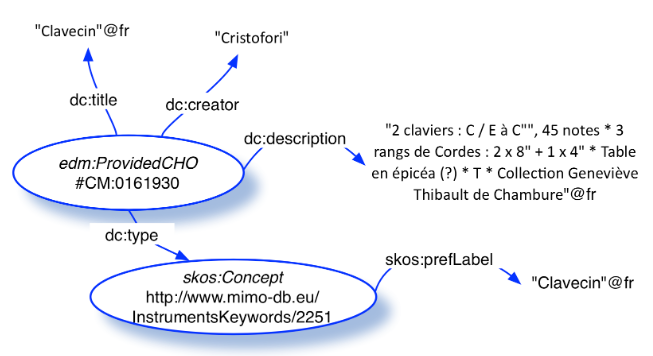
\includegraphics[width=\textwidth]{img/edm-example1.png}

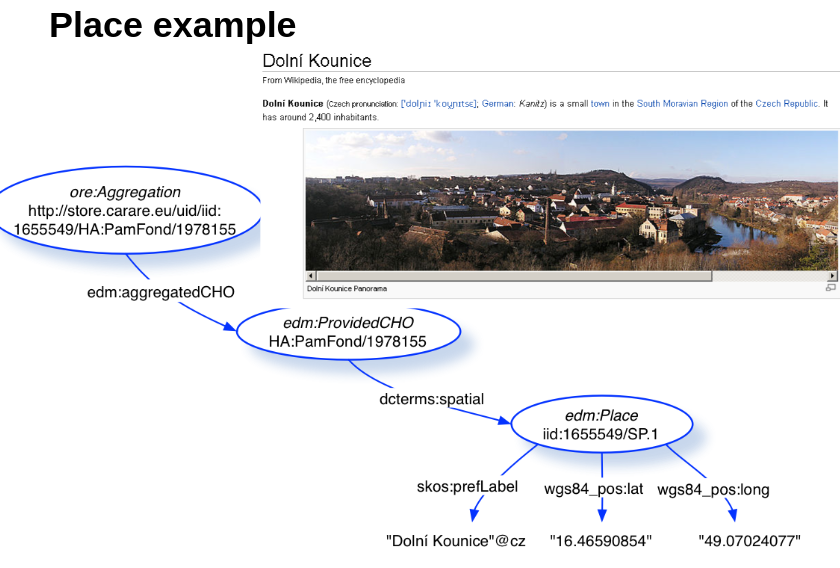
\includegraphics[width=\textwidth]{img/edm-example2.png}

\column{0.48\textwidth}
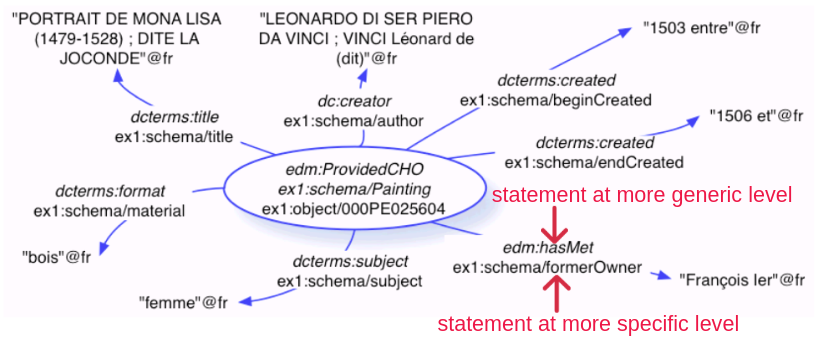
\includegraphics[width=\textwidth]{img/edm-example3.png}

\href{https://pro.europeana.eu/files/Europeana_Professional/Share_your_data/Technical_requirements/EDM_Documentation/EDM_slides_130714.ppt}{(More info.)}
\end{columns}

\end{frame}

%---------------------------------
\begin{frame}[fragile]{Lightweight Information Describing Objects (LIDO)}
\metroset{block=fill}
\begin{columns}
\column{0.48\textwidth}
\begin{block}{LIDO}
\begin{quote}
    Lightweight Information Describing Objects (LIDO) is an\textbf{ XML schema for describing museum or collection objects.} Memory institutions use LIDO for ``exposing, sharing and connecting data on the web''. It can be applied to all kind of disciplines in cultural heritage, e.g. art, natural history, technology, etc. 
    
    LIDO is a specific application of CIDOC CRM. (\href{https://en.wikipedia.org/wiki/LIDO}{Wikipedia})
\end{quote}
\end{block}
\column{0.48\textwidth}\small 
\href{http://gams.uni-graz.at/o:gm.1760}{A postcard (text-bearing object)}

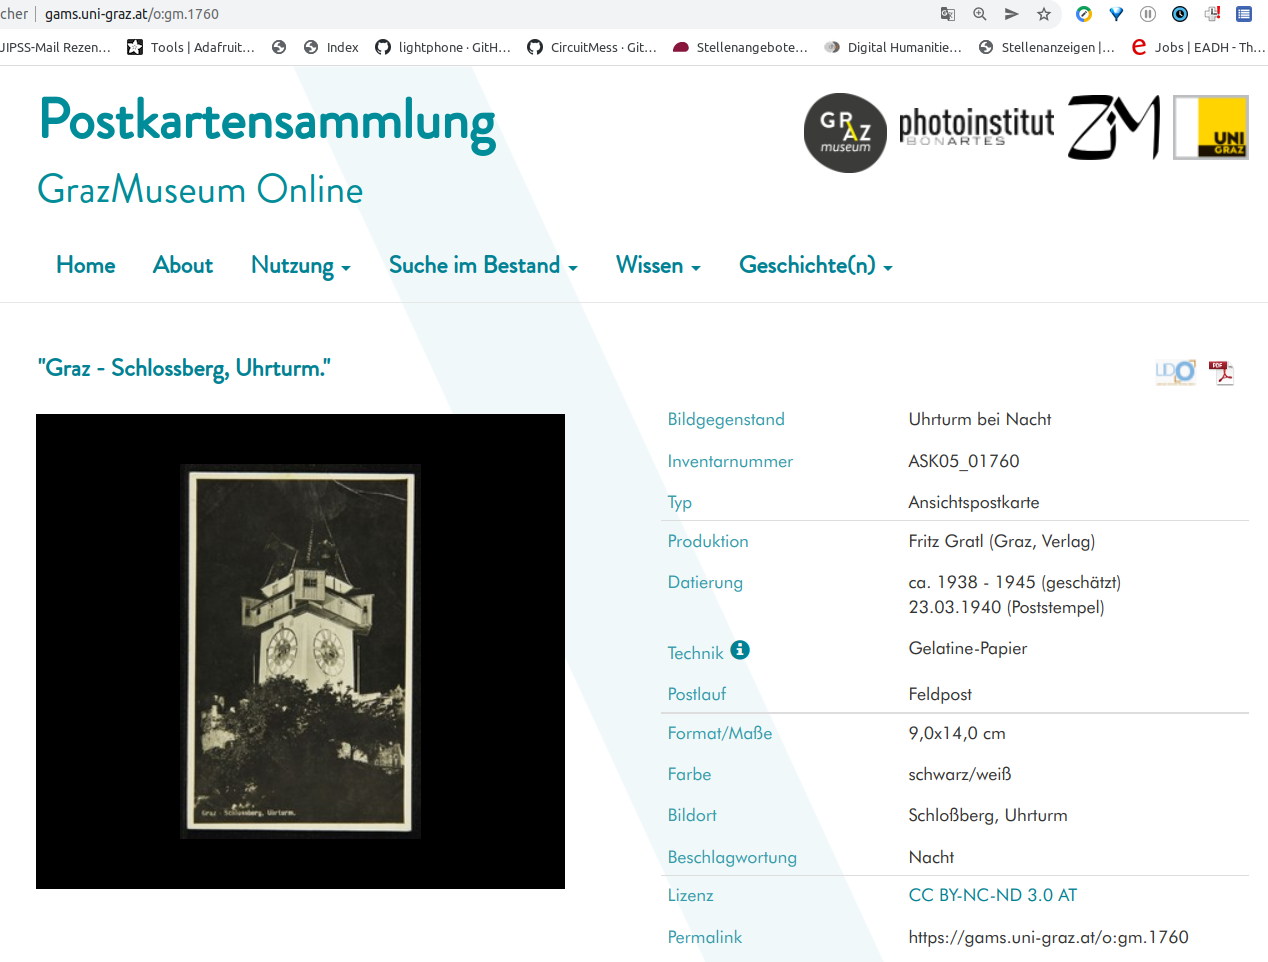
\includegraphics[width=\textwidth]{img/text-bearing-objects.png}

\begin{xmlcode}
<lido:titleWrap>
    <lido:titleSet>
        <lido:appellationValue>
            Chickens and Ducks
        </lido:appellationValue>
    </lido:titleSet>
</lido:titleWrap>
\end{xmlcode}
\end{columns}
\end{frame}


%---------------------------------------------

\begin{frame}[fragile]{LIDO example 1}

{\scriptsize Notice the two namespaces (\texttt{lido:} and \texttt{t:})! }
    
\begin{xmlcode}
<lido:lido 
  xmlns:lido="http://www.lido-schema.org" 
  xmlns:t="http://www.tei-c.org/ns/1.0">
  <lido:lidoRecID lido:type="PID">o:gm.1760</lido:lidoRecID>
  <lido:category>
    <lido:conceptID lido:source="CIDOC" 
                    lido:type="ID">E22</lido:conceptID>
    <lido:term xml:lang="eng">Man-Made Object</lido:term>
    <lido:term lido:label="info:fedora/context:gm">
      Postkartensammlung Online</lido:term>
  </lido:category>
  <lido:descriptiveMetadata xml:lang="deu">
    <lido:objectClassificationWrap>
      <lido:objectWorkTypeWrap>
        <lido:objectWorkType>
          <lido:conceptID lido:source="http://vocab.getty.edu/aat"
            lido:type="ID">300026819</lido:conceptID>
          <lido:term lido:label="info:fedora/context:gm-ansicht">
            Ansichtspostkarte</lido:term>
        </lido:objectWorkType>
      </lido:objectWorkTypeWrap>
    </lido:objectClassificationWrap>
    <!-- to be continued... LIDO is very verbose --->
\end{xmlcode}

\end{frame}

%---------------------------------------------

\begin{frame}[fragile]{LIDO example 2}

\begin{xmlcode}
<!-- continued... --->

    <lido:objectIdentificationWrap>
      <lido:titleWrap>
        <lido:titleSet>
          <lido:appellationValue>Graz - Schlossberg, Uhrturm.
             </lido:appellationValue>
        </lido:titleSet>
      </lido:titleWrap>
      <lido:repositoryWrap>
        <lido:repositorySet lido:type="orgname">
          <lido:repositoryName>
            <lido:legalBodyID lido:source="http://d-nb.info/gnd"
              lido:type="ID">2022740-1</lido:legalBodyID>
            <lido:legalBodyName>
              <lido:appellationValue>GrazMuseum</lido:appellationValue>
            </lido:legalBodyName>
          </lido:repositoryName>
          
    <!-- to be continued... LIDO is very verbose --->
\end{xmlcode}

\end{frame}



%-----------------------------------------------------
\begin{frame}{Internat. Image Interoperability Framework (read: \emph{Triple-I-F})}

\begin{columns}
\column{0.48\textwidth}
\begin{block}{IIIF}
\begin{quote}
    The International Image Interoperability Framework (\protect\url{https://iiif.io/}) defines several application programming interfaces that provide a standardised method of describing and delivering images over the web, as well as ``presentation based metadata'' about structured sequences of images. (\href{https://en.wikipedia.org/wiki/International_Image_Interoperability_Framework}{Wikipedia})
\end{quote}
\end{block}

\column{0.48\textwidth}
\begin{block}{The standard}
\begin{itemize}\footnotesize
    \item proposed in 2011 
    \item 2012: Version 1.0
    \item \textbf{Image API:} URL for viewing the images
    \item \textbf{Presentation API:} standard for describing a sequence of canvases and the images they are represented by as a representation of an object (\emph{manifest}, \texttt{manifest.json})
\end{itemize}
\end{block}
\end{columns}

 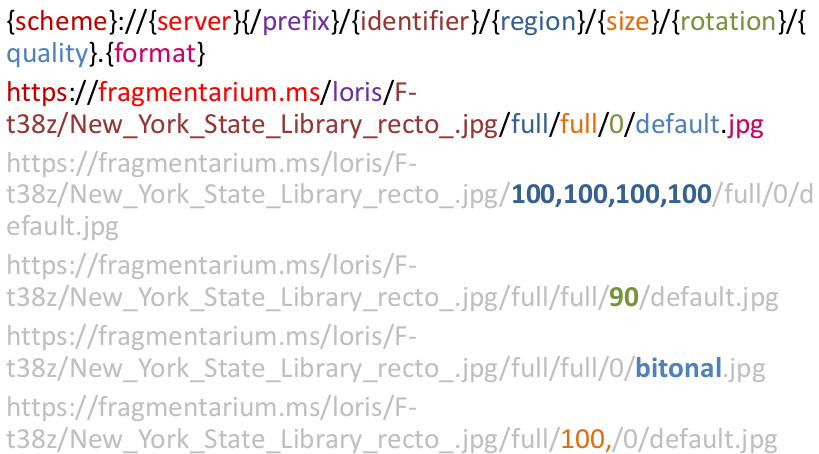
\includegraphics[width=0.7\textwidth]{img/iiif.png}

\end{frame}
%-----------------------------------------------------
\begin{frame}{IIIF Image API}

\begin{columns}
\column{0.48\textwidth}
\begin{block}{region}\footnotesize
defines the rectangular portion of the
underlying image content to be returned
\end{block}

\begin{block}{size}\footnotesize
determines the dimensions to which the
extracted region is to be scaled
\end{block}

\begin{block}{rotation}\footnotesize
 otation parameter specifies mirroring and rotation
\end{block}
\begin{block}{IIIF Presentation API}\footnotesize
\href{https://jubilees.stmarytx.edu/mirador/index.html}{example 1}, 
\href{https://jubilees.stmarytx.edu/iiifp/KB_Collin-36-III-082/manifest.json}{example 2}
\end{block}

\column{0.48\textwidth}
\begin{block}{quality}\footnotesize
determines whether the image is delivered in
color, grayscale or black and white (values: color, gray, bitonal, default)
\end{block} 

\begin{block}{format}\footnotesize
format of the returned image (e.g. jpg, tif, gif, jp2, pdf, webp)
\end{block} 

\begin{block}{Mirador Web Viewer}\footnotesize
Fully featured IIIF Viewer: \protect\url{https://projectmirador.org}
\end{block}


\end{columns}

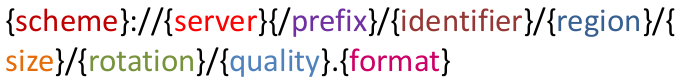
\includegraphics[width=0.9\textwidth]{img/iiif-image-api.png}
\end{frame}


%-----------------------------------------------------


